%\documentclass[a4paper]{article}
%% Language and font encodings
\documentclass[twocolumn,aps,prl]{revtex4-1}
\usepackage[utf8]{inputenc}
\usepackage[spanish, es-tabla]{babel}
\usepackage[T1]{fontenc}
\usepackage{amsmath}
\usepackage{amssymb}
\usepackage{siunitx}
\usepackage{multirow}
\usepackage{float}
\usepackage{enumitem} % enumerar

\sisetup{math-micro=\text{µ},text-micro=µ}

\usepackage[toc,page]{appendix}

%% Sets page size and margins
\usepackage[a4paper,top=1.5cm,bottom=2cm,left=1.7cm,right=1.7cm,marginparwidth=1.75cm]{geometry}

%% Sets caption text size(its bigger than text)
\usepackage{caption}
\captionsetup[figure]{font=small}
\usepackage{subcaption}

%% Useful packages
\usepackage{svg}
\usepackage{epstopdf}
\usepackage{amsmath}
\usepackage{graphicx}
\usepackage[colorlinks=true, allcolors=blue]{hyperref}

\newcommand{\nstar}{n^*} 
\newcommand{\Nstar}{N^*} 

\newcommand*\sepline{%
  \begin{center}
    \rule[1ex]{.5\textwidth}{.5pt}
  \end{center}}

%%%%%%%%%%%%%%%%%%%%%%%%%%%%%%%%%%%%%%%%%%%%%%%%%%%%%%
%%%%%%%%%%%%%%%%%%%%%%%%%%%%%%%%%%%%%%%%%%%%%%%%%%%%%%
%%%%%%%%%%%%%%%%%%%%%%%%%%%%%%%%%%%%%%%%%%%%%%%%%%%%%%
%%%%%%%%%%%%%%%%%%%%%%%%%%%%%%%%%%%%%%%%%%%%%%%%%%%%%%
%%%%%%%%%%%%%%%%%%%%%%%%%%%%%%%%%%%%%%%%%%%%%%%%%%%%%%

\begin{document}

% ██   ██ ███████  █████  ██████
% ██   ██ ██      ██   ██ ██   ██
% ███████ █████   ███████ ██   ██
% ██   ██ ██      ██   ██ ██   ██
% ██   ██ ███████ ██   ██ ██████

\title{Práctico 5}
\author{M. G. Aramayo}
\affiliation{Matemática de sistemas biológicos, Instituto Balseiro}

% \begin{abstract}
% Mete acá las conclusiones.
% \end{abstract}

\maketitle


% ███████╗██╗  ██╗ ██╗
% ██╔════╝╚██╗██╔╝███║
% █████╗   ╚███╔╝ ╚██║
% ██╔══╝   ██╔██╗  ██║
% ███████╗██╔╝ ██╗ ██║
% ╚══════╝╚═╝  ╚═╝ ╚═╝

\section{Resolución Ej 1:}

Se analiza el modelo epidemiológico SIRS, dado por el sistema dinámico:
$$
\left\lbrace
\begin{aligned}
\frac{d s}{d t} & = f_1(s,i,r) = -\beta s i+\frac{1}{\tau_{R}} r \\
\frac{d i}{d t} & = f_2(s,i,r) =\beta s i-\frac{1}{\tau_{I}} i \\
\frac{d r}{d t} & = f_3(s,i,r) =\frac{1}{\tau_{I}} i-\frac{1}{\tau_{R}} r
\end{aligned}
\right.
$$
a poblacion constante, por lo que: $s+i+r =1 $

Los equilibrios del sistema $\left(s^{*}, i^{*}, r^{*}\right)$ se obtienen mediante:

$$
\left\lbrace
\begin{aligned}
f_1(s^*, i^*, r^*) &= 0  \\
f_2(s^*, i^*, r^*) &= 0  \\
f_3(s^*, i^*, r^*) &= 0
\end{aligned}
\right.
\Rightarrow
\left\lbrace
\begin{aligned}
\beta s^* i^* = \frac{1}{\tau_{R}} r^* \\
\beta s^* i^* = \frac{1}{\tau_{I}} i^* \\
\frac{1}{\tau_{I}} i^* = \frac{1}{\tau_{R}} r^*
\end{aligned}
\right.
\Rightarrow
\left\lbrace
\begin{aligned}
i^* &= \frac{\tau_{I}}{\tau_{R}} r^* \\
s^* &= \frac{1}{\tau_{I} \beta}      \\
i^* &= \frac{\tau_{I}}{\tau_{R}} r^* 
\end{aligned}
\right.
$$, con $i \neq 0$

El sistema anterior y la poblacion constante implica que:

$$
i^{*} \quad=\frac{\beta \tau_{I}-1}{\beta\left(\tau_{l}+\tau_{R}\right)}
$$

No se pierde mucho descartando $i^{*}=0$, ese equilibrio no tiene dinamica.


Mediante un analisis lineal es posible demostrar que el sistema presenta oscilaciones amortiguadas. 

Con la condicion de poblacion constante es posible reducir el sistema a uno bidimesional:
$$ \left\lbrace
\begin{aligned}
\frac{d s}{d t} &= f_1(s, i) = -\beta s i+\frac{(1-s-i)}{\tau_{R}} r , \\
\frac{d i}{d t} &= f_2(s, i) = \beta s i-\frac{1}{\tau_{I}} i  
\end{aligned}
\right.
$$
Con su correspondiente matriz jacobiana:
$$
J (s, i) = 
\left(
  \begin{array}{cc}
-\beta i - \frac{1}{\tau_{R}} & -\beta s - \frac{1}{\tau_{R}} \\
 \beta i                     &   \beta s - \frac{1}{\tau_{I}}
  \end{array}
\right)
$$
el analisis lineal requiere obtener los autovalores $\lambda_{1,2}$ de la matriz jacobiana del sistema, la ecuacion caracteristica resulta:

$$
\begin{aligned}
  0 & = \lambda^{2} \\
  \quad & +\lambda\left(\beta i^{*}+\frac{1}{\tau_{R}}-\beta s^{*}+\frac{1}{\tau_{I}}\right) \\
  \quad & +\left(\frac{\beta i^{*}}{\tau_{I}}-\frac{\beta s^{*}}{\tau_{R}}+\frac{1}{\tau_{I} \tau_{R}}+\frac{\beta i^{*}}{\tau_{R}}\right)
\end{aligned}
$$

Para seguir, utilizamos las expresiones del punto de equilibrio $\left(s^{*}, i^{*}\right)$ en función de los parámetros del sistemas. Estas expresiones las encontramos en el apartado anterior. De esta manera, con un poco de álgebra, la ecuación (18) se torna en la ecuación (19):

\sepline

anterior. De esta manera, con un poco de álgebra, la ecuación (18) se torna en la ecuación (19):
$$
\lambda^{2}+\lambda\left(\frac{\beta \tau_{I}-1}{\tau_{l}+\tau_{R}}+\frac{1}{\tau_{R}}\right)+\left(\frac{\beta \tau_{l}-1}{\tau_{l} \tau_{R}}\right) \quad=0
$$
Esta es una ecuación cuadrática de segundo grado que se resuelve fácilmente. Sus dos soluciones, que llamamos $\lambda_{1}, 2$ son:
$$
\left.\lambda_{1,2} \quad=-\frac{1}{2}\left(\frac{\beta \tau_{l}-1}{\tau_{I}+\tau_{R}}+\frac{1}{\tau_{R}}\right) \pm \sqrt{\left(\frac{\beta \tau_{I}-1}{\tau_{I}+\tau_{R}}+\frac{1}{\tau_{R}}\right)^{2}-4\left(\frac{\beta \tau_{I}-1}{\tau_{I} \tau_{R}}\right.}\right)
$$
y corresponden a los dos autovalores que buscamos. El término fuera de la raíz es negativo, dado que:
$$
\left(\frac{\beta \tau_{I}-1}{\tau_{I}+\tau_{R}}+\frac{1}{\tau_{R}}\right) \quad>0
$$
Tras un poco de álgebra, se desprende que esta condición se cumple si y sólo si:
$\beta \tau_{R} \quad>-1$
la cual se satisface trivialmente porque tanto $\beta$ como $\tau_{R}$ son números reales positivos.
de distinto signo, con lo cual habrá un saddle
correspondiente con un punto azul.

\sepline

%**********
\begin{figure*}[ht!]
  \begin{subfigure}[b]{0.49\linewidth}
    \centering
      \centering
      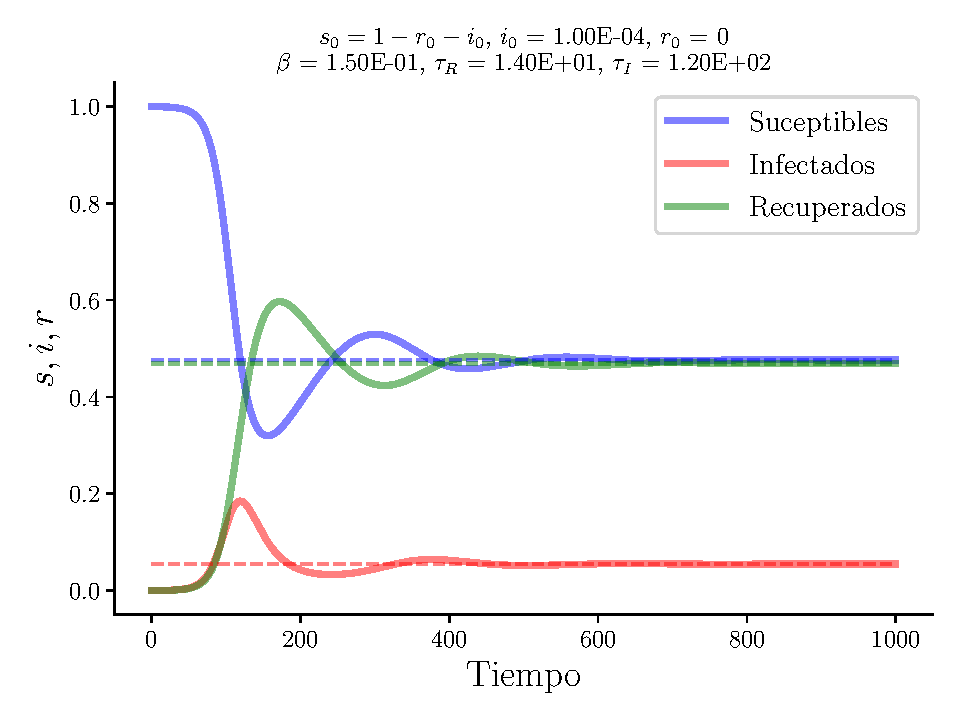
\includegraphics[width = 0.9\textwidth]{figuras/ex01-a-sir.pdf}
      \caption{}
      \label{fig:figuras/ex01-a-sir}
  \end{subfigure}\quad
%   \caption{}
%   %\label{fig:figuras/ex01-a-sir}
% \end{figure*}
% \begin{figure*}[ht!]
%   \centering
  \begin{subfigure}[b]{0.49\linewidth}
      \centering
      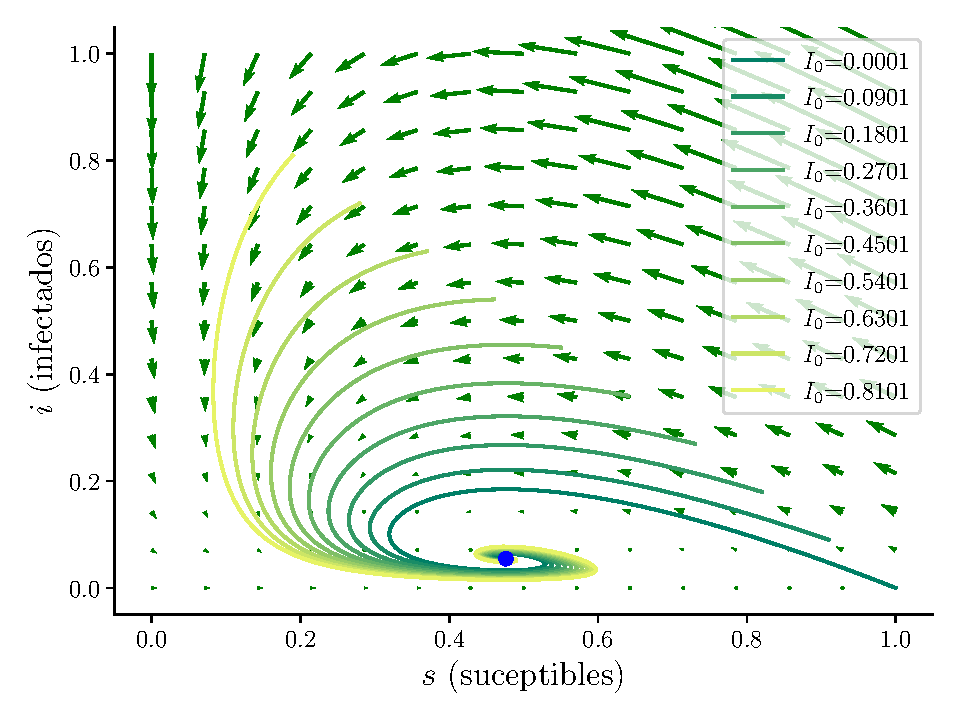
\includegraphics[width = 0.9\textwidth]{figuras/ex01-a-vector.pdf}
      \caption{}
      \label{fig:figuras/ex01-a-vector}
  \end{subfigure}\quad
  % \caption{}
  %\label{fig:figuras/ex01-a-vector}
% \end{figure*}
% \begin{figure*}[ht!]
%   \centering

  \begin{subfigure}[b]{0.49\linewidth}
      \centering
      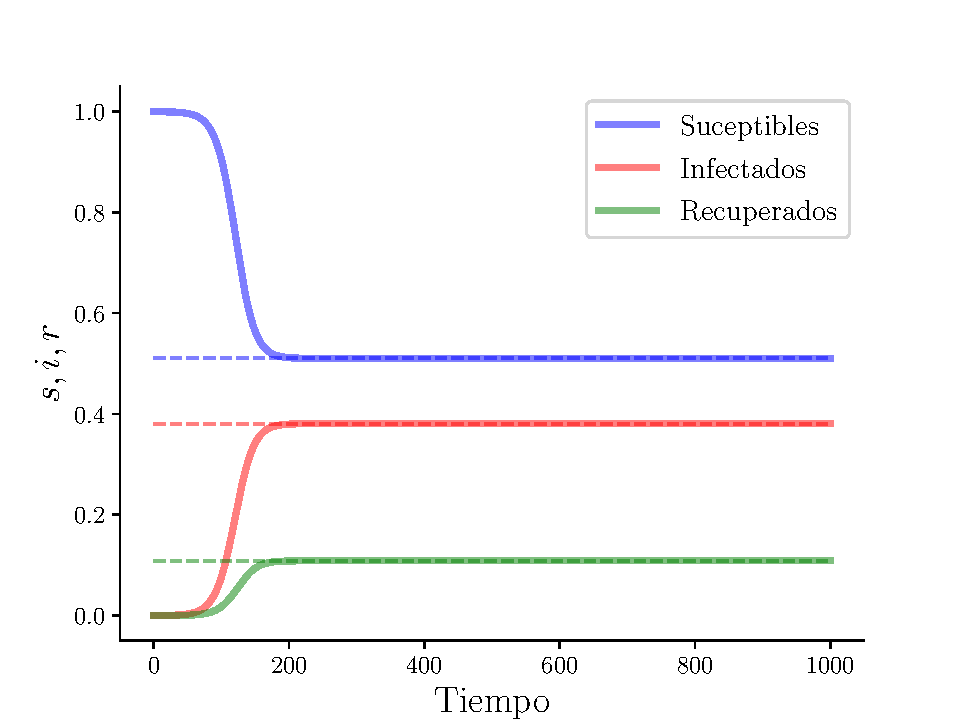
\includegraphics[width = 0.9\textwidth]{figuras/ex01-b-sir.pdf}
      \caption{}
      \label{fig:figuras/ex01-b-sir}
  \end{subfigure}\quad
%   \caption{}
%   %\label{fig:figuras/ex01-b-sir}
% \end{figure*}
% \begin{figure*}[ht!]
%   \centering
  \begin{subfigure}[b]{0.49\linewidth}
      \centering
      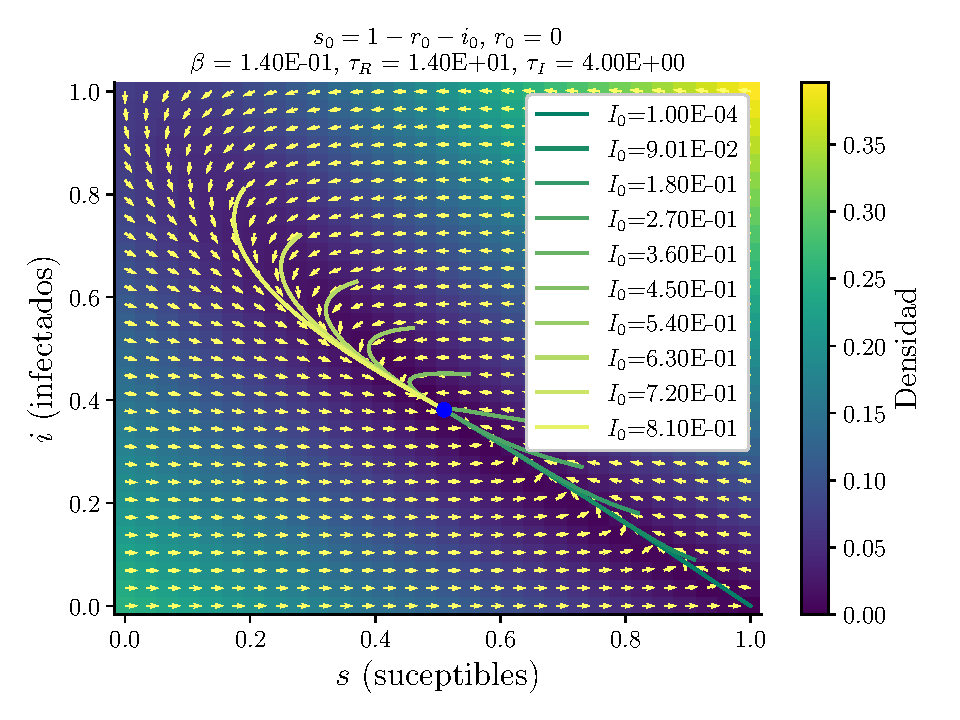
\includegraphics[width = 0.9\textwidth]{figuras/ex01-b-vector.pdf}
      \caption{}
      \label{fig:figuras/ex01-b-vector}
  \end{subfigure}\quad
%   \caption{}
%   %\label{fig:figuras/ex01-b-vector}
% \end{figure*}
% \begin{figure*}[ht!]
%   \centering

  \begin{subfigure}[b]{0.49\linewidth}
      \centering
      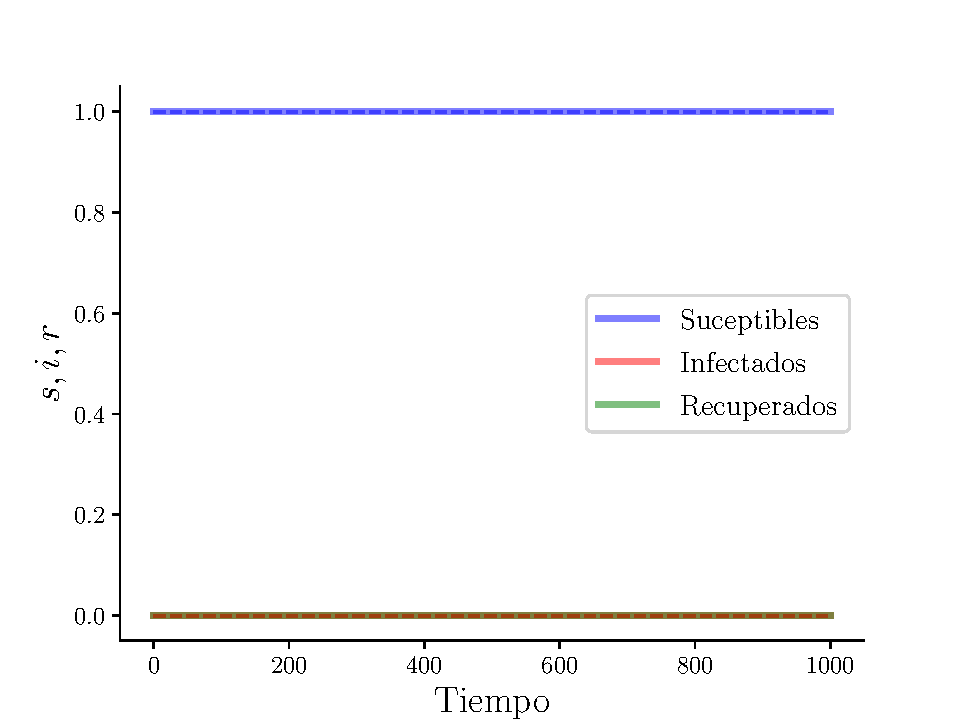
\includegraphics[width = 0.9\textwidth]{figuras/ex01-c-sir.pdf}
      \caption{}
      \label{fig:figuras/ex01-c-sir}
  \end{subfigure}\quad
%   \caption{}
%   %\label{fig:figuras/ex01-c-sir}
% \end{figure*}
% \begin{figure*}[ht!]
%   \centering
  \begin{subfigure}[b]{0.49\linewidth}
      \centering
      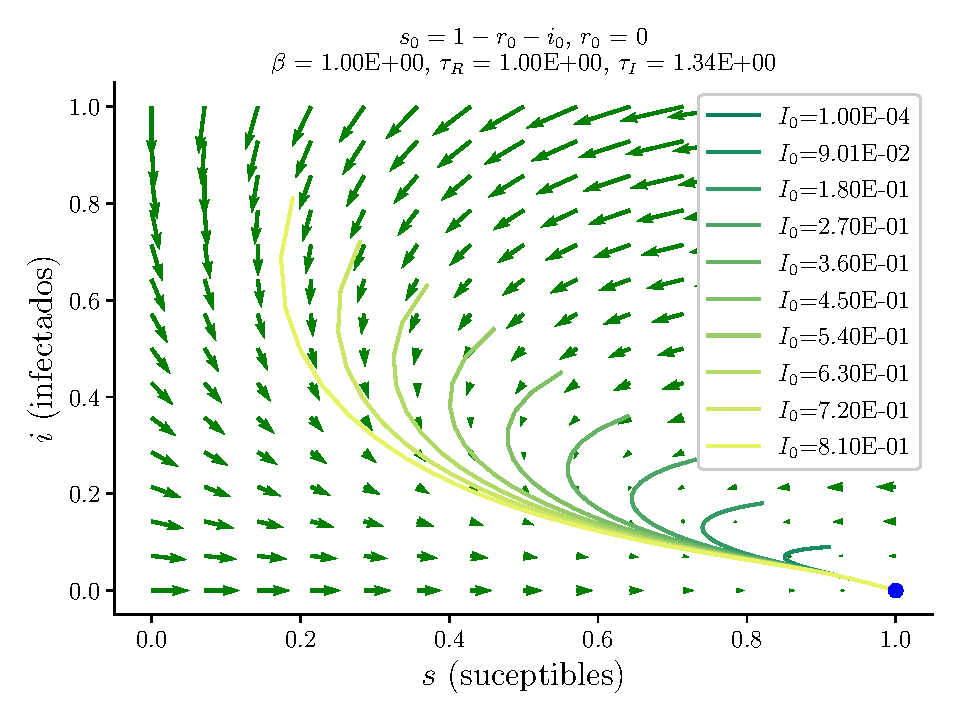
\includegraphics[width = 0.9\textwidth]{figuras/ex01-c-vector.pdf}
      \caption{}
      \label{fig:figuras/ex01-c-vector}
  \end{subfigure}\quad
  \caption{}
  %\label{fig:figuras/ex01-c-vector}
\end{figure*}

% ███████╗██╗  ██╗    ██████╗  
% ██╔════╝╚██╗██╔╝    ╚════██╗
% █████╗   ╚███╔╝      █████╔╝
% ██╔══╝   ██╔██╗     ██╔═══╝ 
% ███████╗██╔╝ ██╗    ███████╗
% ╚══════╝╚═╝  ╚═╝    ╚══════╝

\section{Resolución Ej 2:}

El pico que figura en los datos sin feriados y fines de semana, ocurre el \textbf{2020-10-21}. Tomando datos desde el \textbf{2020-03-05}, se predice que la fecha del pico es \textbf{2020-10-08} luego de 168 dias(24 semanas) de datos. Por esto, se predice la fecha del primer pico con 62 dias de antelacion y con un error de 13 dias. En la Fig. \ref{fig:figuras/ex02-resumen}, se tienen las predicciones que se obtienen para disintos numeros de semanas de datos sobre los cuales se realiza el ajuste. 

% \begin{figure*}[ht!]
%   \centering
%   % \begin{subfigure}[b]{0.9\linewidth}
%       \centering
%       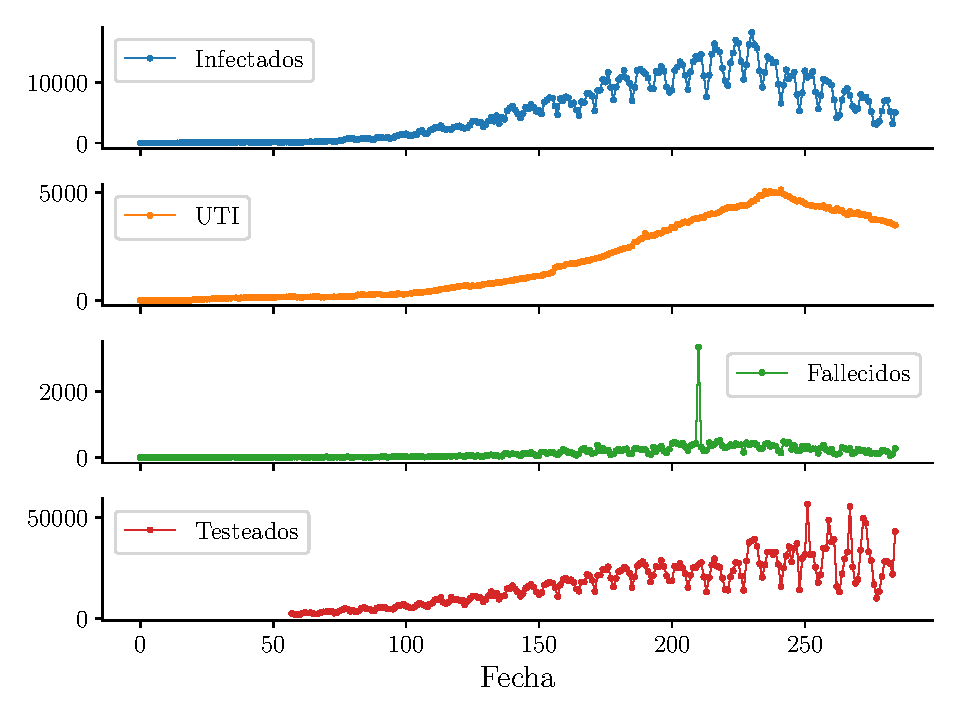
\includegraphics[width = 0.9\textwidth]{figuras/ex02-pico1.pdf}
%       % \caption{}
%       \label{fig:figuras/ex02-pico1}
%   % \end{subfigure}\quad
%   \caption{Graficos }
%   %\label{fig:figuras/ex02-pico1}
% \end{figure*}

\begin{figure*}[ht!]
  \centering
  % \begin{subfigure}[b]{0.33\linewidth}
      \centering
      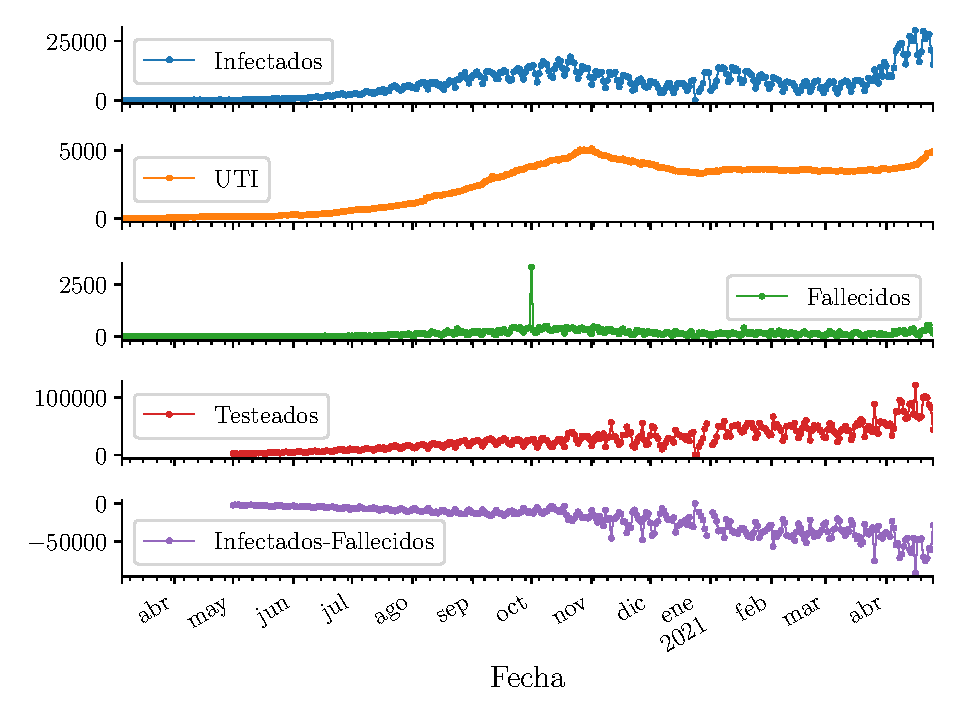
\includegraphics[width = 0.9\textwidth]{figuras/ex02-resumen.pdf}
      % \caption{}
      \label{fig:figuras/ex02-resumen}
  % \end{subfigure}\quad
  \caption{}
  %\label{fig:figuras/ex02-resumen}
\end{figure*}

\begin{figure*}[ht!]
  \centering
  \begin{subfigure}[b]{0.49\linewidth}
      \centering
      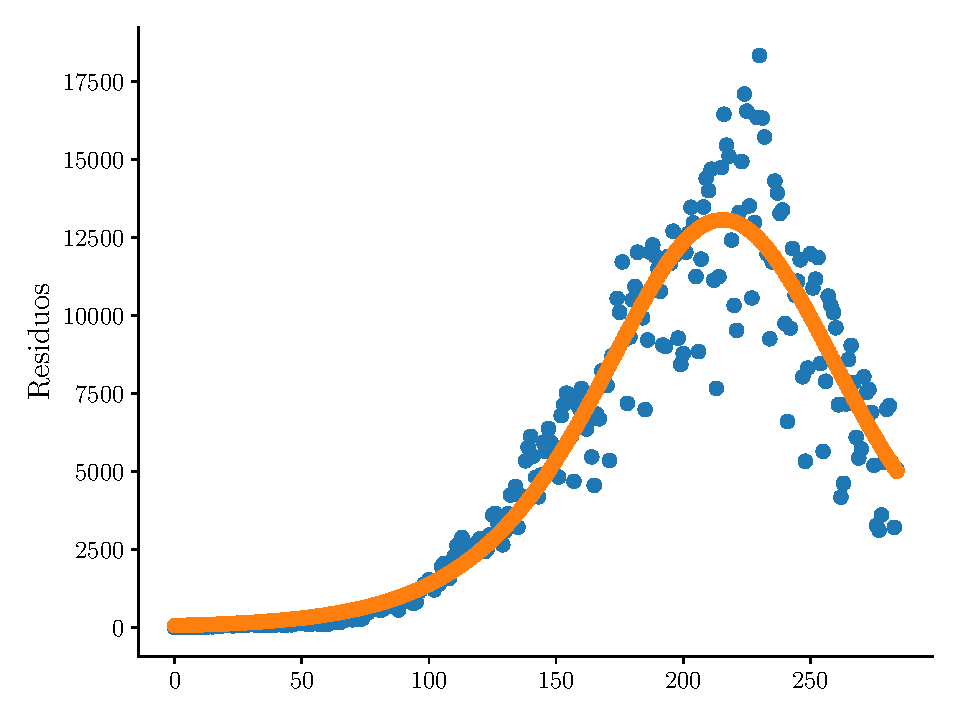
\includegraphics[width = 0.9\textwidth]{figuras/ex02-fit.pdf}
      \caption{}
      \label{fig:figuras/ex02-fit}
  \end{subfigure}\quad
  \begin{subfigure}[b]{0.49\linewidth}
      \centering
      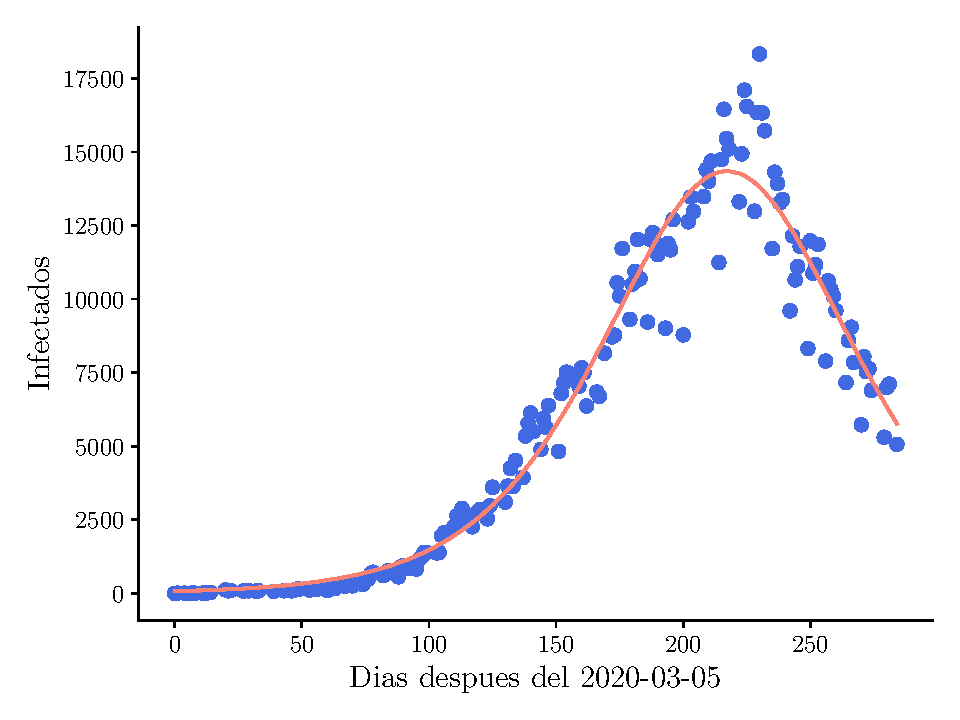
\includegraphics[width = 0.9\textwidth]{figuras/ex02-fit-sin-Finde.pdf}
      \caption{}
      \label{fig:figuras/ex02-fit-sin-Finde}
  \end{subfigure}\quad

  \begin{subfigure}[b]{0.49\linewidth}
      \centering
      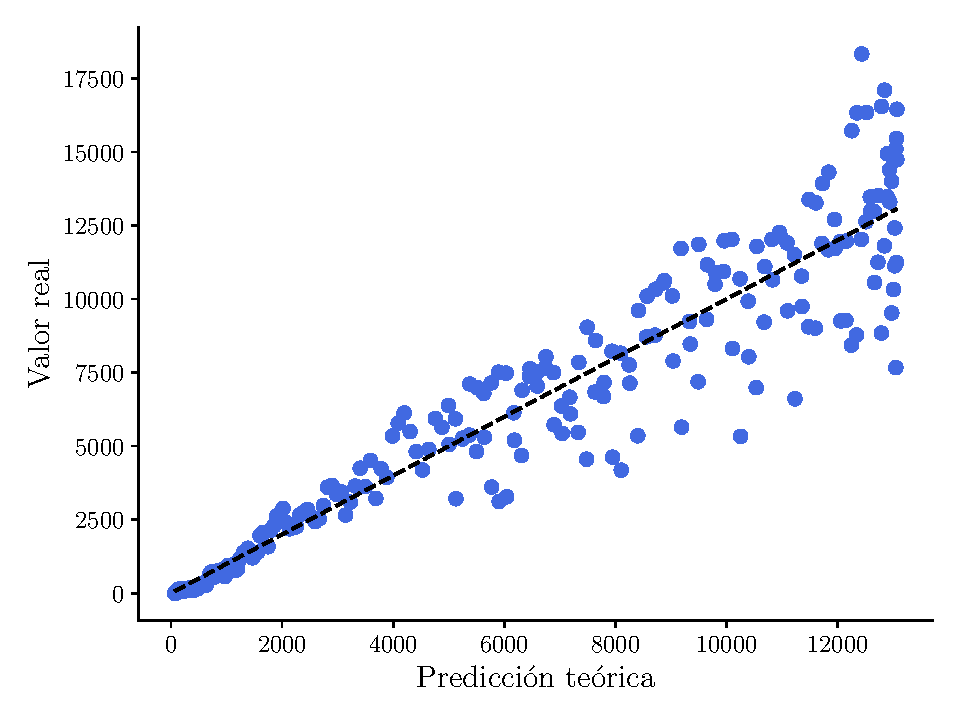
\includegraphics[width = 0.9\textwidth]{figuras/ex02-qq.pdf}
      \caption{}
      \label{fig:figuras/ex02-qq}
  \end{subfigure}\quad
  \begin{subfigure}[b]{0.49\linewidth}
      \centering
      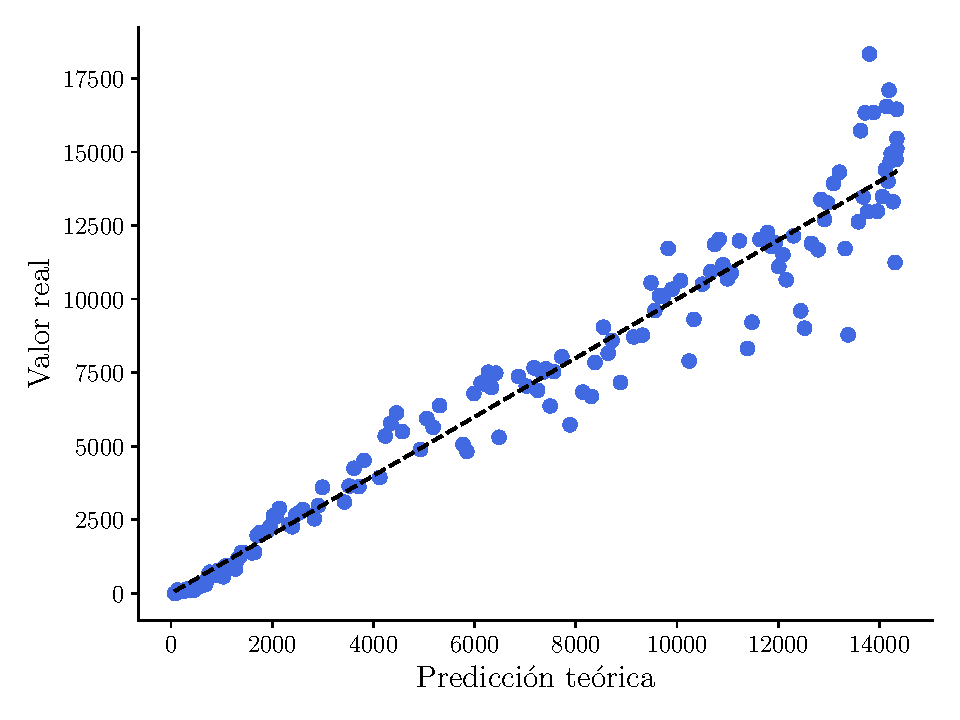
\includegraphics[width = 0.9\textwidth]{figuras/ex02-qq-sin-Finde.pdf}
      \caption{}
      \label{fig:figuras/ex02-qq-sin-Finde}
  \end{subfigure}\quad

  \begin{subfigure}[b]{0.49\linewidth}
      \centering
      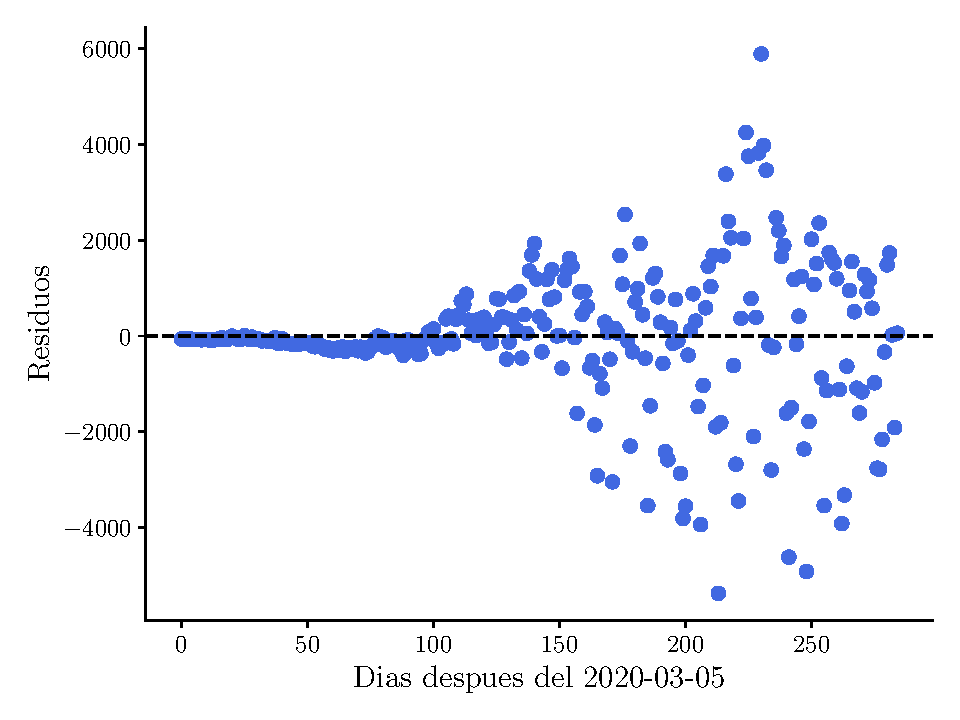
\includegraphics[width = 0.9\textwidth]{figuras/ex02-residuos.pdf}
      \caption{}
      \label{fig:figuras/ex02-residuos}
  \end{subfigure}\quad
  \begin{subfigure}[b]{0.49\linewidth}
      \centering
      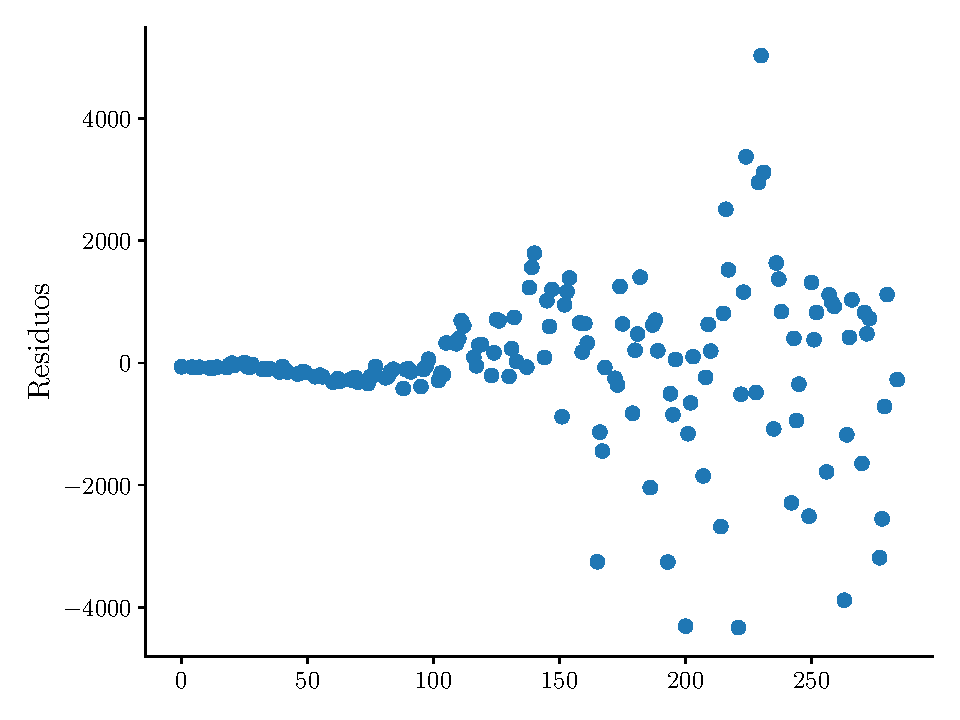
\includegraphics[width = 0.9\textwidth]{figuras/ex02-residuos-sin-Finde.pdf}
      \caption{}
      \label{fig:figuras/ex02-residuos-sin-Finde}
  \end{subfigure}\quad
  \caption{}
  %\label{fig:figuras/ex02-residuos-sin-Finde}
\end{figure*}

\begin{figure*}[ht!]
  \centering
  % \begin{subfigure}[b]{0.33\linewidth}
      \centering
      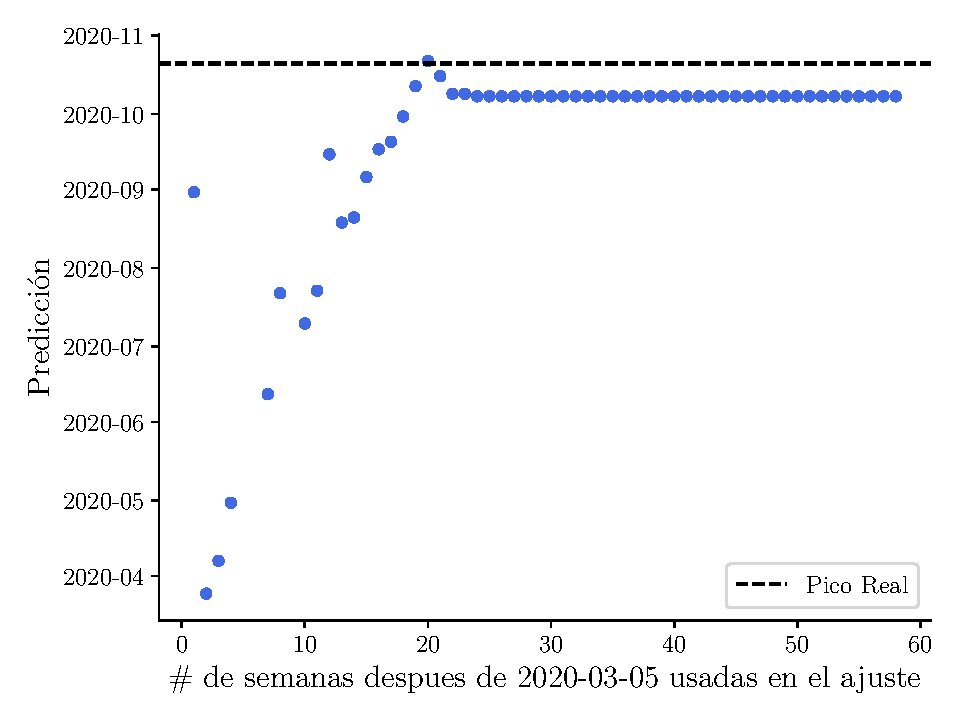
\includegraphics[width = 0.9\textwidth]{figuras/ex02-prediccion-semanas.pdf}
      % \caption{}
      \label{fig:figuras/ex02-resumen}
  % \end{subfigure}\quad
  \caption{}
  %\label{fig:figuras/ex02-resumen}
\end{figure*}

% \begin{figure*}[ht!]
%   \centering
%   \begin{subfigure}[b]{0.33\linewidth}
%       \centering
%       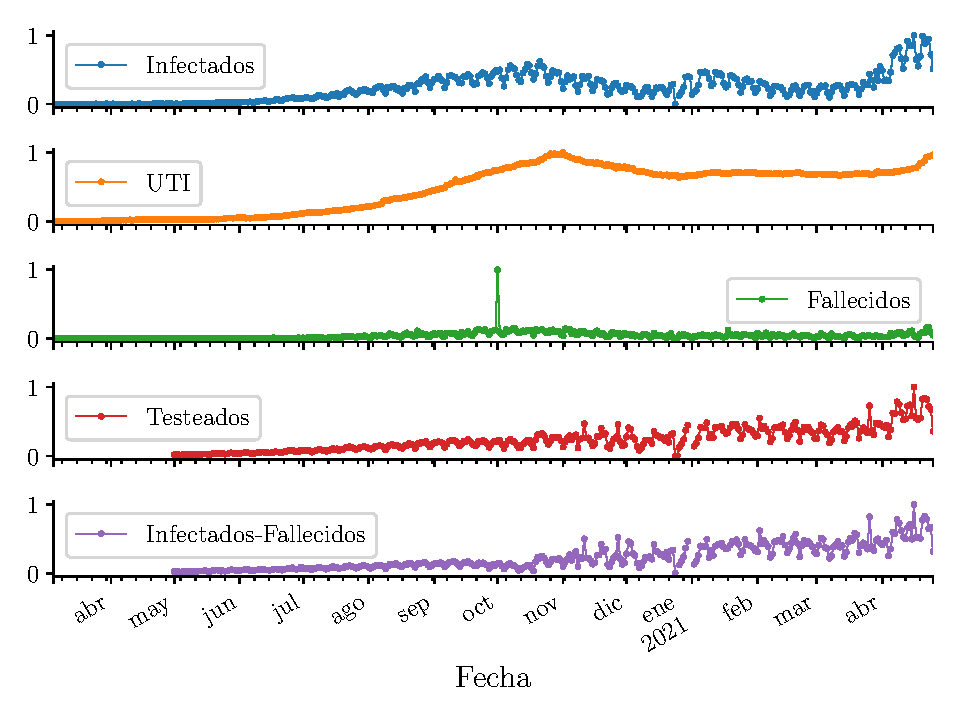
\includegraphics[width = 0.9\textwidth]{figuras/ex02-resumen-normalizado.pdf}
%       \caption{}
%       \label{fig:figuras/ex02-resumen-normalizado}
%   \end{subfigure}\quad
%   \caption{}
%   %\label{fig:figuras/ex02-resumen-normalizado}
% \end{figure*}

% \begin{figure*}[ht!]
%   \centering
%   \begin{subfigure}[b]{0.33\linewidth}
%       \centering
%       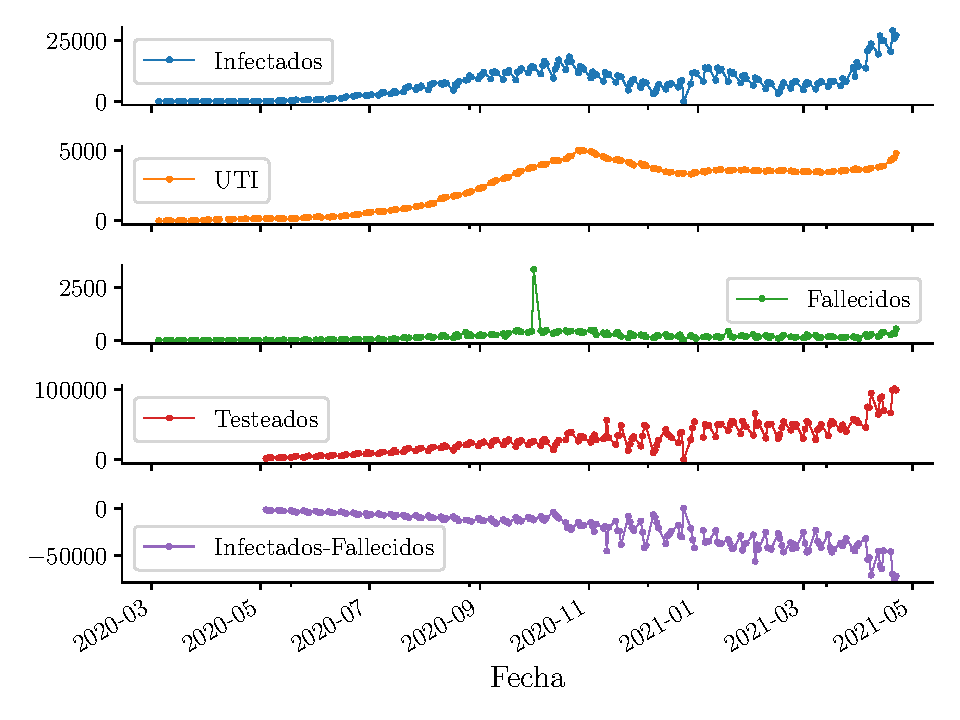
\includegraphics[width = 0.9\textwidth]{figuras/ex02-sin-Finde.pdf}
%       \caption{}
%       \label{fig:figuras/ex02-sin-Finde}
%   \end{subfigure}\quad
%   \caption{}
%   %\label{fig:figuras/ex02-sin-Finde}
% \end{figure*}
% \begin{figure*}[ht!]
%   \centering
%   \begin{subfigure}[b]{0.33\linewidth}
%       \centering
%       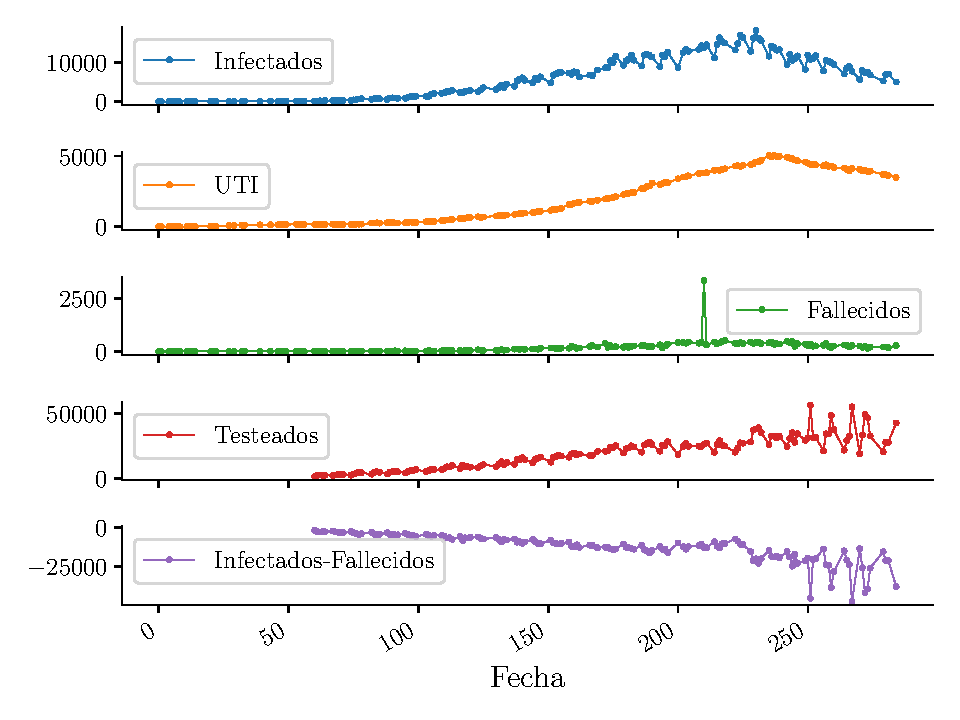
\includegraphics[width = 0.9\textwidth]{figuras/ex02-sin-Finde-pico1.pdf}
%       \caption{}
%       \label{fig:figuras/ex02-sin-Finde-pico1}
%   \end{subfigure}\quad
%   \caption{}
%   %\label{fig:figuras/ex02-sin-Finde-pico1}
% \end{figure*}
%**********


% \bibliography{sample}

\end{document}

% ███    ██  ██████  ████████  █████  ███████
% ████   ██ ██    ██    ██    ██   ██ ██
% ██ ██  ██ ██    ██    ██    ███████ ███████
% ██  ██ ██ ██    ██    ██    ██   ██      ██
% ██   ████  ██████     ██    ██   ██ ███████


% ████████ ██    ██ ██████   ██████  ███████
%    ██     ██  ██  ██   ██ ██    ██ ██
%    ██      ████   ██████  ██    ██ ███████
%    ██       ██    ██      ██    ██      ██
%    ██       ██    ██       ██████  ███████

% atomico
% volumen
% parametro
% mantenia
% dielectrico
% perdida
% ferroelectrico
% difractograma
% difractometro
% minimo
% maximo
% tension
% conversion
% aislacion
% medicion
% resolucion
% funcion
% transicion
% correccion
% activacion
% correlacion
% tipico X
% habia  X
% agrego X
